\documentclass[conference]{IEEEtran}

%% DOCUMENT FORMATTING
\usepackage[ngerman]{babel}
\usepackage{csquotes}
\usepackage{geometry}

%% Hyperlinks
\usepackage{hyperref}

%% GRAPHICS
\usepackage{graphicx}

% CITATION
\usepackage{acronym}

\usepackage[style=ieee, maxcitenames=2, mincitenames=1]{biblatex}
\addbibresource{sources.bib}

\usepackage{fancyhdr}
\pagestyle{fancy}
\fancyhf{}
\fancyfoot[C]{\thepage}
\renewcommand{\headrulewidth}{0pt}

\def\BibTeX{{\rmfamily B\kern-.05em{\scshape i\kern-.025em b}\kern-.08em
    T\kern-.1667em\lower.7ex\hbox{E}\kern-.125emX}}

\begin{document}
\title{Generatives Design\\
\large \ \\ \large Wie beeinflusst generatives Design die Gestaltungsprozesse in der Designbranche?}

\author{
  \IEEEauthorblockN{Alexandros Loukaridis}
  \IEEEauthorblockA{\textit{MatNr. 1000730} \\
  92loal1bif@hft-stuttgart.de}

  \and

  \IEEEauthorblockN{Valentin Franco}
  \IEEEauthorblockA{\textit{MatNr. 380094} \\
  91frva1bif@hft-stuttgart.de}
}

\maketitle

\thispagestyle{plain} % Seitennummerierung für das Titelblatt
\pagestyle{plain} % Seitennummerierung für die restlichen Seiten
\pagenumbering{roman} % Seitennummerierung mit römischen Zahlen
\setcounter{page}{1} % Setzt die Seitennummerierung auf 1

\begin{abstract}

    Diese Seminararbeit untersucht den Einfluss des Generativen Designs auf kreative Gestaltungsprozesse in der Designbranche. Die zentrale Fragestellung lautet: Wie beeinflusst das Generative Design den Entscheidungsprozess und die kreative Intuition der Designer? Um diese Frage zu beantworten, werden verschiedene Methoden des Generativen Designs untersucht, darunter parametrisches Design, algorithmisches Design, evolutionäre Algorithmen, prozedurale Generierung, Simulation und Analyse, Machine Learning und Künstliche Intelligenz, generative Algorithmen sowie datengesteuertes Design.
    
    Im Rahmen dieser Seminararbeit werden die grundlegenden Konzepte und Eigenschaften des Generativen Designs erläutert. Dabei liegt der Fokus auf mathematischen Modellen, Regelsystemen und Algorithmen, die zur Beschreibung und Manipulation von formalen und ästhetischen Eigenschaften von Designs verwendet werden. Es werden Fallbeispiele und Anwendungen des Generativen Designs in verschiedenen Bereichen wie Architektur, Produktgestaltung, Grafikdesign, Kunst, Modedesign, Industriedesign sowie Medizin und Gesundheitswesen untersucht.
    
    Die Ergebnisse dieser Untersuchung zeigen, dass das Generative Design einen signifikanten Einfluss auf die kreativen Gestaltungsprozesse hat. Es ermöglicht Designern, effizienter zu arbeiten, Materialersparnisse zu erzielen und innovative Lösungen zu generieren. Durch die Integration von automatisierten Prozessen und algorithmischen Methoden eröffnet das Generative Design neue Wege der Gestaltung, die über traditionelle Designansätze hinausgehen.
    
    Die Folgerungen aus dieser Seminararbeit sind vielfältig. Das Generative Design bietet Potenziale für eine effizientere Gestaltung, die Reduzierung des Materialverbrauchs, die Förderung von Innovationen und eine hohe Anpassungsfähigkeit. Es ermöglicht es Designern, verschiedene Variationen und Optionen zu erkunden und maßgeschneiderte Lösungen für unterschiedliche Nutzerbedürfnisse zu entwickeln. Die Erkenntnisse dieser Arbeit haben Implikationen für die Designpraxis und bieten Anwendungsmöglichkeiten in verschiedenen Bereichen.
    
    Insgesamt liefert diese Seminararbeit ein umfassendes Verständnis für das Generative Design und seine Auswirkungen auf die Designbranche. Sie bietet eine Grundlage für die Diskussion über die Zukunft der kreativen Gestaltungsprozesse und zeigt Wege auf, wie das Generative Design in der Praxis angewendet werden kann, um innovative Lösungen zu generieren.

\end{abstract}

\section{Grundlagen des generativen Designs}
\subsection*{Definition}
Das Generative Design ist ein innovativer Ansatz, bei dem Algorithmen und computergestützte Methoden in den Gestaltungsprozess integriert werden. Es ermöglicht Designern, mithilfe vordefinierter Regeln und Parametern automatisch Variationen und Iterationen von Designs zu generieren (Siehe \autoref{chap:paramDesign}). Im Zentrum steht die Idee, den Computer als kreativen Partner einzubeziehen, um komplexe und innovative Lösungen zu entwickeln, die über traditionelle manuelle oder konventionelle Ansätze hinausgehen.

Eine wichtige Methode im Generativen Design ist die Anwendung parametrischer Modelle. Diese Modelle beschreiben mathematische Zusammenhänge und Regelsysteme, die sowohl die formale als auch ästhetische Eigenschaften von Designs beschreiben und manipulieren können. Durch den Einsatz von Algorithmen und automatisierten Prozessen können Designer effizienter arbeiten und schnell verschiedene Variationen und Optionen erkunden, um neue Perspektiven zu gewinnen und innovative Lösungen zu entwickeln.

\subsection*{Materialersparnisse und Ressourcenoptimierung im Generativen Design}
Ein bedeutendes Ziel des Generativen Designs liegt in den potenziellen Materialersparnissen und der Ressourcenoptimierung. Durch die Integration algorithmischer Methoden und parametrischer Modelle kann das Generative Design dazu beitragen, effizientere und ressourcenschonendere Designs zu entwickeln.

Durch den Einsatz generativer Designwerkzeuge können Designer komplexe Strukturen und Formen optimieren, um Materialverschwendung zu minimieren. Das Generative Design berücksichtigt Belastungen, Spannungen und andere physikalische Anforderungen und gestaltet Designs so, dass sie die benötigte Festigkeit und Stabilität aufweisen, während unnötiges Material entfernt wird. Dadurch können erhebliche Materialersparnisse erzielt werden.

Darüber hinaus eröffnet das Generative Design Möglichkeiten für die Entwicklung von Leichtbaustrukturen, bei denen Material nur dort platziert wird, wo es benötigt wird. Dies führt zu einer erheblichen Reduzierung des Materialverbrauchs und kann zu Gewichtseinsparungen führen, was insbesondere in Bereichen wie der Luft- und Raumfahrt, der Automobilindustrie und der Architektur von großer Bedeutung ist.

Ein weiterer Aspekt ist die Optimierung der Materialwahl. Durch die Fähigkeit des Generativen Designs, komplexe Optimierungen und Simulationen durchzuführen, können Designer alternative Materialien und Materialkombinationen untersuchen, um die Effizienz und Nachhaltigkeit der Designs weiter zu verbessern. Dies ermöglicht es, umweltfreundlichere Materialien einzusetzen und den Einsatz von Ressourcen zu optimieren.

Die Integration von Generativem Design in den Gestaltungsprozess kann somit erhebliche Vorteile hinsichtlich Materialersparnis und Ressourcenoptimierung bieten, was zu nachhaltigeren und effizienteren Designlösungen führt. \autocite*{20}

\subsection*{Historischer Überblick}
Der historische Überblick des Generativen Designs reicht bis in die 1960er und 1970er Jahre zurück, als erste Experimente mit computergestützter Gestaltung durchgeführt wurden. Zu dieser Zeit begannen Designer und Forscher, den Einsatz von Algorithmen und computergestützten Methoden zu erkunden, um kreative Prozesse zu unterstützen.

In den folgenden Jahrzehnten wurden erhebliche Fortschritte in der Computertechnologie und der Algorithmik erzielt, was zu einer breiteren Anwendung generativer Designmethoden führte. Insbesondere mit dem Aufkommen leistungsfähiger Computer und der Entwicklung spezialisierter Designsoftware wurde das Potenzial des Generativen Designs weiter ausgeschöpft.

Heutzutage ist generatives Design in verschiedenen Bereichen der Gestaltung verbreitet. Es findet Anwendung in der Architektur, Produktgestaltung, Grafikdesign und Kunst, Modedesign sowie im Industriedesign. Dabei werden spezifische generative Designmethoden verwendet, um die jeweiligen Anforderungen und Herausforderungen in den einzelnen Bereichen zu bewältigen. \autocite*{18}

\subsection*{Rolle von KI in Generativen Design}
Künstliche Intelligenz (\ac{ki}) spielt eine entscheidende Rolle im generativen Design, da sie die Fähigkeiten von Designern erweitert und den kreativen Prozess unterstützt. Durch den Einsatz von KI-Technologien wie maschinellem Lernen und Deep Learning können Designalgorithmen große Mengen an Daten analysieren, Muster erkennen und neue Designlösungen generieren. KI ermöglicht es, komplexe Zusammenhänge und Anforderungen zu berücksichtigen und gleichzeitig innovative und effiziente Designs zu schaffen.

Ein wichtiger Aspekt ist die Optimierung von Designs. KI-basierte Algorithmen können die Topologieoptimierung unterstützen (Siehe \autoref{chap:topology}), um Materialien und Strukturen zu identifizieren, die die gewünschten Leistungsmerkmale erfüllen. Durch die Simulation und Bewertung verschiedener Designoptionen kann KI helfen, optimale Lösungen zu finden, die herkömmlichem Design möglicherweise entgehen würden.

Darüber hinaus ermöglicht KI auch die Integration von Benutzerpräferenzen und Designvorgaben. Durch das Lernen aus Nutzerfeedback und historischen Daten können KI-Systeme personalisierte Designempfehlungen geben und den Designprozess auf die individuellen Bedürfnisse und Vorlieben der Benutzer abstimmen.

Die Rolle von KI im generativen Design geht jedoch über die Automatisierung und Unterstützung von Designaufgaben hinaus. Sie eröffnet auch neue Möglichkeiten für kreative Exploration und die Schaffung neuartiger Designs. KI kann dabei helfen, Designräume zu erforschen, unkonventionelle Lösungen zu identifizieren und innovative Konzepte zu generieren, die traditionelle Designansätze herausfordern.

Insgesamt trägt KI dazu bei, den Designprozess effizienter, vielfältiger und kreativer zu gestalten. Sie unterstützt Designer dabei, neue Ideen zu generieren, Designräume zu erkunden und optimale Lösungen zu finden, die den Anforderungen und Präferenzen der Benutzer gerecht werden. Durch die enge Verbindung von KI und generativem Design eröffnen sich spannende Perspektiven für die Gestaltung zukünftiger Produkte und Systeme. \autocite*{21} \autocite*{22}

\subsection*{Benötigte Technologien für Generatives Design}
Generatives Design erfordert oft große Rechenleistung und Speicherplatz, insbesondere bei komplexen Projekten. Aus diesem Grund ist Cloud-Computing eine geeignete Lösung, da es skalierbare Ressourcen in Form von virtuellen Maschinen und Speicherplatz bietet. Durch die Nutzung von Cloud-Computing können Designer auf leistungsstarke Recheninfrastruktur zugreifen und große Datenmengen effizient verarbeiten.

Ein weiterer wichtiger Aspekt ist das High-Performance Computing (HPC). Da generatives Design rechenintensiv ist und viele Iterationen und Optimierungsschritte erfordert, können HPC-Systeme mit Mehrkernprozessoren und paralleler Verarbeitung die Rechenzeiten erheblich verkürzen. Diese Systeme können entweder in einer Cloud-Infrastruktur oder lokal betrieben werden, je nach den Anforderungen des Projekts.

Generatives Design benötigt eine Menge an Daten, wie zum Beispiel topografische Informationen \autoref{chap:topology}, Gebäudeparameter und Materialdaten. Daher ist eine robuste Infrastruktur für das Datenmanagement und die Integration von entscheidender Bedeutung. Dies umfasst die Einrichtung von Datenbanken, die Entwicklung von Datenpipelines und die Integration von Daten aus verschiedenen Quellen, um effektiv mit Daten umgehen zu können. Da große Unternehmen oft an verschiedenen Standorten verteilt sind, ist eine gute Netzwerkinfrastruktur notwendig. 

Ein weiterer wichtiger Aspekt ist die Versionierung und Zusammenarbeit. Bei generativem Design ist es entscheidend, den Überblick über die verschiedenen Designiterationen zu behalten und eine nahtlose Zusammenarbeit zwischen den Teammitgliedern zu ermöglichen. Hier kommen Versionierungssysteme und kollaborative Plattformen zum Einsatz, die die Verwaltung und Zusammenarbeit an gemeinsamen Projekten ermöglichen. Diese bieten eine Historie und erleichtern die Koordination zwischen Teams. \autocite*{23}



\section{Methoden des Generativen Designs}
Unter dem Oberbegriff des generativen Designs sind verschiedene Methoden zu finden, die sich teilweise stark voneinander unterscheiden. Je nach Branche und Designziel werden unterschiedliche Methoden angewendet. Im Folgenden werden einige aktuelle Designmethoden näher beschrieben.

\subsection*{Parametrisches Design}
Parametrisches Design ist eine Methode, bei der Modelle auf einer Reihe von Parametern basieren. Diese Parameter sind variabel und können Eigenschaften wie Größe, Form, Proportionen, Materialien und andere designrelevante Merkmale eines Objekts oder einer Struktur repräsentieren. Bei der Anwendung des parametrischen Designs werden zunächst die Parameter festgelegt, die den Raum der möglichen Designs definieren. Anschließend werden Algorithmen oder Regeln entwickelt, die diese Parameter beeinflussen und miteinander in Beziehung setzen. Durch die Manipulation dieser Parameter können Designer verschiedene Variationen und Iterationen des Designs erzeugen. Der große Vorteil des parametrischen Designs liegt in seiner Flexibilität und Effizienz. Indem die Designentscheidungen auf Parameter abgebildet werden, können Änderungen an einem Parameter automatisch zu Änderungen im gesamten Design führen. Dies ermöglicht eine schnelle Exploration verschiedener Designoptionen und eine einfache Anpassung an veränderte Anforderungen.Darüber hinaus ermöglicht das parametrische Design auch die Optimierung von Designs. Durch die Verwendung von Optimierungsalgorithmen können Designer bestimmte Ziele oder Kriterien festlegen, die das Design erfüllen soll. Der Algorithmus sucht dann automatisch nach den besten Parametereinstellungen, um diese Ziele zu erreichen. Parametrisches Design wird vor allem in Branchen eingesetzt, die die Entwicklung komplexer und maßgeschneiderter Designs erfordern und auf spezifische Anforderungen zugeschnitten werden müssen wie in der Architektur oder im Produktdesign.\autocite{2}

\subsection*{Evolutionäre Algorithmen}
Diese Designmethode ist von den Prinzipien der biologischen Evolution inspiriert. Sie ermöglicht die automatisierte Generierung und Optimierung von Designs, indem eine vorher festgelegte Population von Designs erzeugt und iterativ weiterentwickelt wird.
Der Startpunkt ist die erste Population, die aus einer zufälligen Auswahl möglicher Designs basierend auf einem zufälligen Satz von Parametern besteht. Diese Designs werden entweder vom Designer oder von einer KI mit einem \textit{Fitness-Wert} versehen. Alternativ kann der Designer eine eigens programmierte Fitnessfunktion verwenden, in der er die Kriterien und Ziele festlegt, die das Enddesign erfüllen soll. Dadurch wird kein menschlicher Input mehr benötigt, bis ein Ergebnis erzielt wird. Anhand der bewerteten Designs wird dann die zweite Generation von Designs erstellt. Diese zweite Generation erbt die Eigenschaften der Designs aus der ersten Generation, die einen hohen \textit{Fitness-Wert} hatten. Dieser Prozess wird wiederholt, bis ein zufriedenstellendes Ergebnis erreicht ist. Mit jeder Iteration werden die Designs immer besser an die Anforderungen angepasst.\autocite{3}

\subsection*{Generative Adversarial Networks (GANs)}
Bei \ac*{GANs} handelt es sich um zwei konkurrierende Künstliche Neuronale Netzwerke (\ac*{KNN}), die im Austausch miteinander stehen. Ein \ac*{KNN} ist dafür zuständig, reale Designs zu generieren und wird auch als Generator bezeichnet. Das andere \ac*{KNN} ist für die Klassifizierung dieser Designs zuständig und wird als Diskriminator bezeichnet. Der Diskriminator bewertet die generierten Designs nach ihrem Realismus und gibt dieses Feedback an den Generator zurück. Um diese Bewertung durchführen zu können, muss der Diskriminator logischerweise auf realen und generierten Bildern trainiert sein, um den Unterschied zwischen ihnen mit hoher Wahrscheinlichkeit einschätzen zu können. Wie bei den evolutionären Algorithmen verbessern sich die Ergebnisse, die das \ac*{GAN} liefert, mit der Anzahl der Iterationen.\autocite{4}\autocite{11}


\section{Anwendungen des Generativen Designs}
\subsection*{Anwendungen in Branchen}
Architektur: Generatives Design wird in der Architektur eingesetzt, um innovative Gebäudestrukturen zu entwerfen. Durch die Verwendung von algorithmischen Methoden und parametrischen Modellen können Architekten komplexe und effiziente Gebäudekonzepte entwickeln. Das Generative Design ermöglicht es, verschiedene Parameter wie Materialverbrauch, Energieeffizienz und Raumoptimierung zu berücksichtigen und so nachhaltige Architektur zu fördern.

Produktgestaltung: Im Bereich der Produktgestaltung eröffnet das Generative Design neue Möglichkeiten zur Entwicklung maßgeschneiderter und funktional optimierter Produkte. Durch den Einsatz von Algorithmen und automatisierten Prozessen können Designer Variationen von Produkten generieren und diese an individuelle Kundenanforderungen anpassen. Dadurch können einzigartige und effiziente Produkte mit verbesserten Leistungsmerkmalen geschaffen werden.

Automobilindustrie: In der Automobilindustrie wird das Generative Design verwendet, um leichtere und dennoch stabile Fahrzeugkomponenten zu entwickeln. Durch die Integration von algorithmischen Optimierungsmethoden können Ingenieure komplexe Strukturen gestalten, die mit herkömmlichen Designansätzen schwer umzusetzen wären. Das Ergebnis sind Fahrzeugkomponenten, die sowohl Gewicht einsparen als auch die Fahrzeugleistung verbessern, beispielsweise durch bessere Aerodynamik oder höhere strukturelle Festigkeit.

\subsection*{Generativ Design Software von Autodesk und Ablauf}

Generative Design (GD) Tools werden zunehmend in verschiedenen technischen Bereichen eingesetzt. Dabei handelt es sich um Softwaretools, die künstliche Intelligenz (KI) Methoden und Algorithmen verwenden, um Designprobleme zu lösen. Ein Unternehmen, das sich stark auf die Entwicklung solcher GD-Tools und deren Integration in herkömmliche CAD-Umgebungen konzentriert hat, ist Autodesk. Autodesk hat das Projekt "Dreamcatcher" gestartet, das sich seit 2014 der Entwicklung von GD-Tools widmet. Nach fünf Jahren Entwicklung wurde die erste Version der kommerziellen GD-Software veröffentlicht. Das GD-Tool von Autodesk heißt "Generative Design" und ist in Fusion 360, einem parametrischen CAD-Modellierer, integriert. 

Generative Design von Autodesk ermöglicht die Optimierung der Form eines Bauteils, um statische strukturelle Belastungen zu erfüllen. Cloud-Computing-Funktionen werden genutzt, um mehrere Finite-Elemente-Analysen durchzuführen und ein akzeptables Ergebnis innerhalb einer akzeptablen Zeitspanne zu erhalten. Im Gegensatz zur Topologieoptimierung erfordert Generative Design weniger Anpassungen und Einrichtungsphasen und ist somit für eine breitere Anwendung zugänglich. Dennoch erfordert die bewusste Anwendung von GD-Tools bestimmte Fähigkeiten, die derzeit noch nicht vollständig entwickelt und weit verbreitet sind. 



\begin{figure}[h]
    \begin{minipage}{0.5\textwidth}
      \centering
      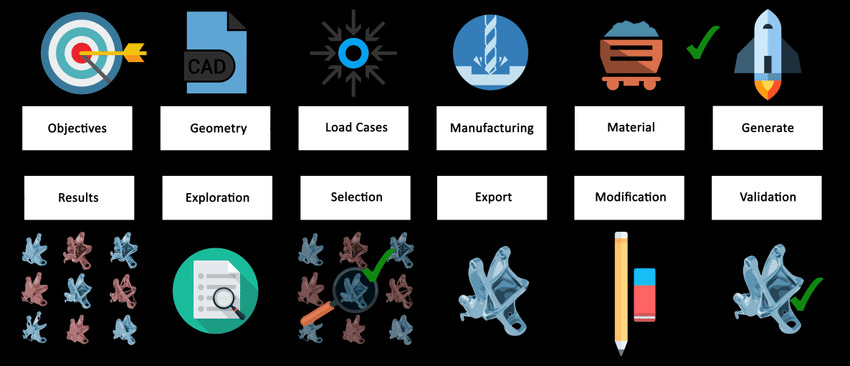
\includegraphics[width=\textwidth]{./images/Autodesk-Generative-Design-Framework.jpeg}
    \end{minipage}
    \caption{Autodesk Prozessablauf}
    \label{fig:meinbild}
  \end{figure}
  

Autodesk Generative Design bietet verschiedene Phasen im Arbeitsablauf, darunter:

1. Ziele: Der Benutzer kann zwischen zwei Optionen wählen, entweder die Masse zu minimieren oder die Steifigkeit zu maximieren. In beiden Fällen wird ein Sicherheitsfaktor benötigt. Bei Auswahl der zweiten Option muss der Benutzer auch eine Zielmasse angeben, die die Optimierung erreichen soll.

2. Geometrie: Der Benutzer definiert die Bereiche, die von der Optimierung unverändert bleiben sollen (Erhaltungsbereiche) und die Bereiche, die leer bleiben müssen (Hindernisbereiche). Im Gegensatz zum klassischen Ansatz der Topologieoptimierung erfordert Generative Design keine Definition eines Ausgangsvolumens (Designraum), das schrittweise ausgehöhlt wird. Die Optimierung kann mit einer plausiblen Ausgangsform (Starting Shape) gestartet werden, was jedoch optional ist.

3. Lastfälle: Generative Design unterstützt Kräfte, Drücke und Lagerlasten. Es können auch die Schwerkraft berücksichtigt werden. Verfügbar sind festgelegte, festgeklemmte und reibungsfreie Einschränkungen. Mehrere Lastfälle können vom Solver berücksichtigt werden, jedoch können keine dynamischen Bedingungen eingeführt werden. Alle Lasten und Einschränkungen müssen auf die Erhaltungsbereiche angewendet werden.

4. Fertigungsbeschränkungen: Der Benutzer kann Fertigungsbeschränkungen angeben, um die Optimierung auf Formen auszurichten, die mit einem bestimmten Herstellungsprozess (Additive Fertigung, 5-Achs-Fräsen, 3-Achs-Fräsen) hergestellt werden können, um die Produktionskosten für die Bauteil

fertigung zu reduzieren.

5. Material: Derzeit können nur linear-elastische Modelle verwendet werden. Generative Design ermöglicht jedoch die gleichzeitige Auswahl von bis zu zehn Materialien in einer einzigen Analyse.

6. Eingabeprüfung und Berechnung: Generative Design überprüft, ob alle erforderlichen Informationen vorhanden sind. Wenn dies der Fall ist, werden die Optimierung und die Analysen auf externen Servern mithilfe von Cloud-Computing durchgeführt, nachdem eine festgelegte Gebühr (Cloud-Credits) bezahlt wurde.

7. Ergebnisse: Sobald die Ergebnisse auf dem lokalen Computer heruntergeladen sind, stehen sie dem Benutzer zur Verfügung. Die Ergebnisse können nach mechanischen und physikalischen Eigenschaften dargestellt werden.

8. Exploration: Generative Design bietet eine dedizierte Umgebung mit Visualisierungswerkzeugen, um die Ergebnisse geordnet darzustellen und dem Benutzer bei der Identifizierung der besten Lösung zu helfen.

9. Auswahl: Der Benutzer wählt das Design aus, das am besten zu den gewünschten Anforderungen passt, und exportiert es aus der Visualisierungsumgebung.

10. Export: Das Design wird isoliert und für weitere Änderungen für den Benutzer verfügbar gemacht. Die CAD-Geometrie des Teils wird in die Modellierungsumgebung von Fusion 360 importiert. Für den Export von Designs aus der Visualisierungsumgebung fallen zusätzliche Kosten an.

11. Modifikation: Nach dem Export des Designs muss es mit herkömmlichen CAD-Tools bearbeitet werden, um Fehler zu beheben, die typischerweise in komplexen Formen mit mehreren B-REP-Oberflächen auftreten. Dies ist auch bei Topologieoptimierungen erforderlich, bei denen die tessellierten Formen, die durch die Optimierung erzeugt werden, bearbeitet und optimiert werden müssen, um die Fertigung zu ermöglichen.

12. Validierung: Die Leistungsfähigkeit der exportierten Form muss durch zusätzliche Finite-Elemente-Analysen validiert werden, um die endgültigen mechanischen Eigenschaften des Teils zu bewerten.

\subsection*{Fallbeispiel Heydar Aliyev Centre}
Für das Heydar Aliyev Centre wurde die Software Rhino 3D verwendet. Rhino ist eine 3D-Modellierungssoftware, die sich durch ihre Vielseitigkeit und ihre Fähigkeit zur Generierung komplexer Formen auszeichnet.

\begin{figure}[h]
    \begin{minipage}{0.5\textwidth}
      \centering
      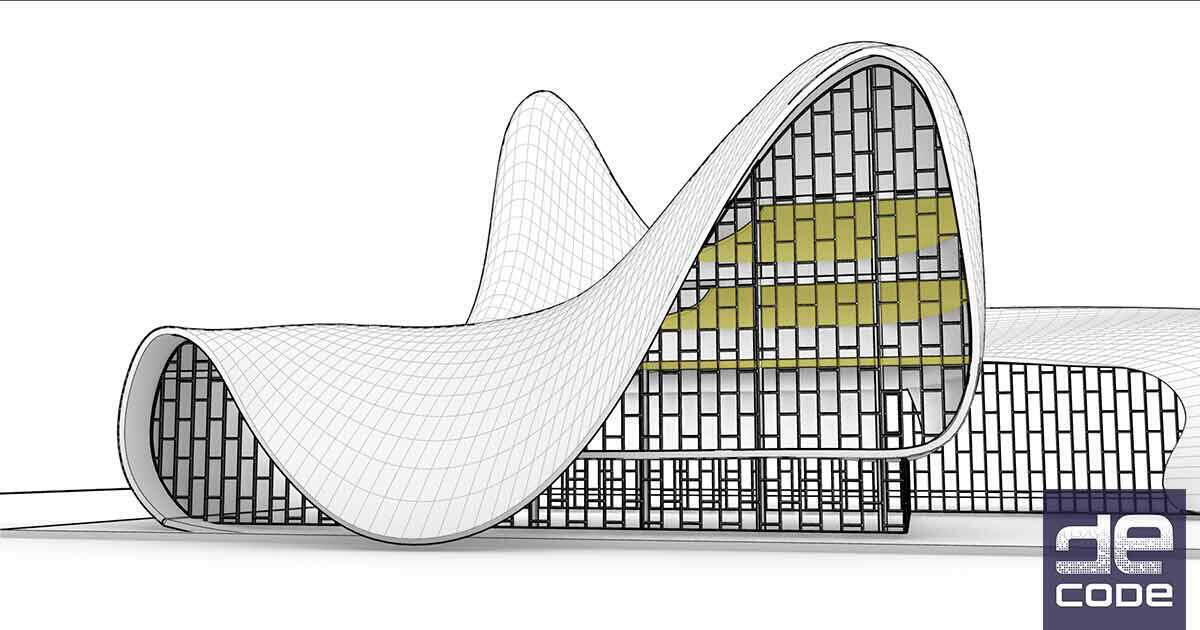
\includegraphics[width=\textwidth]{./images/DE_Rh_lvl1_baku.jpg}
    \end{minipage}
    \caption{Heydar Aliyev Centre}
    \label{fig:meinbild}
  \end{figure}

  Das Heydar Aliyev Centre in Baku ist ein architektonisches Meisterwerk von Zaha Hadid. Es vereint Kunst, Kultur und Geschichte und beeindruckt mit seinen fließenden Formen und innovativen Raumgestaltungen.

  Bei der Gestaltung wurde generatives Design verwendet, um die organischen Kurven und fließenden Formen des Gebäudes zu schaffen. Durch den Einsatz von computergesteuerten Algorithmen konnte das Design-Team verschiedene Parameter und Kriterien festlegen, wie beispielsweise Raumfunktionen, Nutzungsanforderungen, ästhetische Präferenzen und strukturelle Stabilität.

  Basierend auf diesen Parametern konnte das System unzählige mögliche Designs generieren und bewerten. Dabei wurden Aspekte wie räumliche Effizienz, natürliche Belichtung, Zugänglichkeit und visuelle Harmonie berücksichtigt. Das generative Design ermöglichte es den Architekten, schnell eine Vielzahl von Variationen zu erforschen und diejenigen auszuwählen, die am besten den Anforderungen entsprachen.
  
  Das Ergebnis war ein einzigartiges und faszinierendes architektonisches Konzept, das ohne den Einsatz von generativem Design möglicherweise nicht realisierbar gewesen wäre. Das Heydar Aliyev Centre zeigt, wie computergesteuerte Designmethoden neue Horizonte eröffnen und zu außergewöhnlichen architektonischen Kreationen führen können.
  
  Generatives Design hat nicht nur zur Schaffung eines ikonischen Gebäudes beigetragen, sondern es hat auch die Effizienz und Nachhaltigkeit des Designs verbessert. Durch die Berücksichtigung von Faktoren wie Energieeffizienz und optimierte Raumnutzung konnte das Heydar Aliyev Centre eine umweltfreundliche und ressourcenschonende Architektur realisieren.

\section{Herausforderungen und Zukunftsaussichten}
\subsection*{Ethische und rechtliche Aspekte}
Im Rahmen des Reproduktionsdesigns treten verschiedene ethische und rechtliche Fragen auf, die in diesem Abschnitt erörtert werden. Eine der zentralen ethischen Fragen betrifft die Urheberschaft und Originalität generativ gestalteter Werke. Da generatives Design auf Algorithmen und computergenerierten Prozessen basiert, stellt sich die Frage, ob der Designer oder der Algorithmus als Urheber des Werkes oder Designs anzusehen ist. Dies wirft Fragen zu geistigen Eigentumsrechten und den damit verbundenen Rechten und Pflichten auf.  
 Ein weiterer ethischer Aspekt betrifft die Auswirkungen reproduktiver Gestaltung auf Arbeit und Berufsleben. Automatisierung und algorithmische Erstellung von Designlösungen können sich auf traditionelle kreative Berufe auswirken und zum Verlust von Arbeitsplätzen führen. Ethische Verantwortung berücksichtigt die gesellschaftlichen Auswirkungen von Veränderungen  und findet geeignete Lösungen für die Umschulung von Mitarbeitern oder die Schaffung neuer Arbeitsfelder. 
 Darüber hinaus können Datenschutz- und Informationssicherheitsprobleme im Zusammenhang mit reproduktivem Design auftreten. Das Sammeln und Verarbeiten von Daten zur Verbesserung von Zuchtalgorithmen kann besorgniserregend sein, insbesondere wenn personenbezogene Daten ohne deren Zustimmung  verwendet werden. Es ist wichtig, betriebliche Methoden und Best Practices zu entwickeln, um den Schutz personenbezogener Daten und die Einhaltung  der Datenschutzgesetze sicherzustellen. Rechtlich kann es Fragen zur Haftung und Verantwortung für Fehler oder Schäden im Zusammenhang mit reproduktiver Gestaltung geben. Wer trägt die Schuld, wenn ein Algorithmus oder eine KI-basierte Software versagt? Es ist wichtig, einen klaren rechtlichen Rahmen zu schaffen, um potenzielle Streitigkeiten zu vermeiden und die Verantwortung angemessen zu verteilen. 
 Die Berücksichtigung der ethischen und rechtlichen Aspekte des Reproduktionsdesigns ist sehr wichtig, um die potenziellen Auswirkungen dieser Technologie zu verstehen und geeignete Richtlinien und Vorschriften zum Schutz der Rechte und Interessen sowohl der Designer als auch der Gesellschaft als Ganzes zu entwickeln. Nur mit einem verantwortungsvollen Vorgehen können die Chancen des reproduktiven Designs genutzt und potenzielle Risiken minimiert werden.

 \subsection*{Technologische Entwicklung}
 Generatives Design steht in engem Zusammenhang mit technologischen Entwicklungen, die das Potenzial haben, diese Designpraxis weiter voranzutreiben und zu verbessern. In diesem Abschnitt werden einige der wichtigsten technologischen Trends und Entwicklungen im Zusammenhang mit reproduktivem Design untersucht. 
 1. Fortschritte in der Rechenleistung: Mit  technologischen Fortschritten und kontinuierlich steigender Rechenleistung werden komplexe Generierungsalgorithmen und Simulationen schneller und effizienter. Dies eröffnet neue Möglichkeiten zur Designerstellung und -optimierung in Echtzeit und ermöglicht die Verarbeitung großer Datenmengen für noch genauere Ergebnisse.  2. Künstliche Intelligenz (KI): Die Integration künstlicher Intelligenztechnologien wie maschinelles Lernen und Deep Learning im Bereich reproduktives Design eröffnet spannende Perspektiven. Mithilfe künstlicher Intelligenz können generative Algorithmen lernen, Muster zu erkennen, Vorlieben von Menschen zu verstehen und auf Basis dieser Erkenntnisse optimierte Modelle zu erstellen. Auf künstlicher Intelligenz basierende generative Systeme können kontinuierlich lernen und sich an Designanforderungen anpassen. 
 3. 3D-Druck und additive Fertigung: Fortschritte in der 3D-Drucktechnologie ermöglichen die Erstellung generativ gestalteter Objekte und Strukturen direkt aus digitalen Modellen. Dies eröffnet neue Möglichkeiten zur Realisierung komplexer und individueller Designlösungen, die mit herkömmlichen Produktionsmethoden nur schwer zu realisieren wären. Generative Pläne können speziell auf die Anforderungen des 3D-Drucks zugeschnitten werden, um optimale Ergebnisse zu erzielen.  
 4. Virtual Reality (VR) und Augmented Reality (AR): VR- und AR-Technologien eröffnen neue Möglichkeiten zur Visualisierung und Interaktion mit generativen Designs. Designer können virtuelle Umgebungen nutzen, um ihre Ideen zu visualisieren und zu testen,  bevor sie sie physisch umsetzen. AR ermöglicht es, generative Designlösungen in die reale Welt zu projizieren und  in verschiedenen Kontexten zu betrachten, was wiederum das Design-Feedback verbessert und den Designprozess rationalisiert. 
 5. Datenanalyse und -visualisierung: Der Zugriff auf große Datenmengen und  Fortschritte in der Datenanalyse ermöglichen die Erstellung von Plänen auf der Grundlage umfangreicher Daten. Durch die Analyse von Benutzerdaten, Trends und anderen relevanten Informationen können generative Algorithmen personalisierte Modelle erstellen und auf individuelle Vorlieben und Anforderungen reagieren.  Diese technologische Entwicklung eröffnet neue Möglichkeiten für reproduktives Design und wird voraussichtlich zur Integration und Verbesserung dieser Designpraxis führen. Sie bieten mehr Kreativität, Effizienz und Innovation in verschiedenen Anwendungsbereichen und haben großen Einfluss auf die Zukunft des reproduktiven Designs.

 \subsection*{Potenzial für Innovationen und kreative Lösungen}
 Generatives Design birgt ein großes Potenzial für Innovationen und kreative Lösungen in verschiedenen Bereichen. Die Kombination aus algorithmischer Intelligenz, Datenanalyse und automatischer Generierung ermöglicht es Designern, traditionelle Designgrenzen zu verschieben und innovative Ansätze zu entwickeln. 
 Erhebliches Potenzial liegt in der Effizienz und Optimierungsfähigkeit reproduktiver Designs. Durch die Integration komplexer Parameter und Anforderungen in den Designprozess können Designs optimiert werden. Algorithmen und Simulationen ermöglichen die Anpassung von Effizienz, Festigkeit oder anderen Kriterien, was zu individuelleren und funktionaleren Produkten und Strukturen führt.  Ein weiteres Potenzial ist die individuelle Gestaltung des Designs. Mithilfe von Datenanalysen und maschinellem Lernen können generative Designlösungen personalisierte Designs erstellen, die auf individuelle Bedürfnisse und Vorlieben zugeschnitten sind. Kunden können einzigartige Produkte erhalten, die auf bestimmte Parameter wie Körpergröße oder individuelle Vorlieben zugeschnitten sind. Dies ermöglicht ein individuelles Benutzererlebnis und eröffnet neue Möglichkeiten im Bereich Custom Design. 
 Generatives Design unterstützt auch die kreative Erkundung. Mithilfe von Algorithmen und Computermodellen können Designer mit vielen Variationen und Möglichkeiten experimentieren. Es fördert den kreativen Entdeckungsprozess und ermöglicht die Erforschung ungewöhnlicher Ideen  und die Entdeckung neuer ästhetischer Ausdrucksformen. 
 Darüber hinaus bietet generatives Design das Potenzial für nachhaltiges Design. Durch die Optimierung des Materialeinsatzes, der Gewichtsreduzierung und der Energieeffizienz tragen generative Designlösungen dazu bei, Ressourcen zu schonen und den ökologischen Fußabdruck zu minimieren. Die Kombination von generativem Design mit nachhaltigen Materialien und Produktionsmethoden kann zu innovativen Lösungen für umweltbewusstes Design führen. Ein weiteres Potenzial des generativen Designs ist Zusammenarbeit und Co-Kreation. Kreative Tools und Plattformen ermöglichen Designern, Ingenieuren und anderen Fachleuten die Zusammenarbeit. Es fördert den Gedankenaustausch, die Kombination unterschiedlicher Expertisen und die Schaffung interdisziplinärer Lösungen. 
 Die Möglichkeiten für Innovationen und kreative Lösungen im Reproduktionsdesign sind umfangreich. Durch den Einsatz von Algorithmen, Datenanalyse und Automatisierung können Designprozesse verbessert und neue Wege zur Gestaltung der Zukunft geschaffen werden. Generative Planung ermöglicht eine effiziente und personalisierte Planung, fördert nachhaltiges Denken und eröffnet Möglichkeiten zur Zusammenarbeit und Zusammenarbeit zwischen verschiedenen Abteilungen.

\section{Fazit}
\subsection*{Zusammenfassung der Ergebnisse}

In dieser Seminararbeit wurde ausführlich auf das Thema Reproduktionsdesign eingegangen. Die Grundlagen des Reproduktionsdesigns wurden definiert und die historische Entwicklung vorgestellt. Es wurden auch verschiedene Methoden des generativen Designs eingeführt, darunter parametrisches Design, algorithmisches Design, evolutionäre Algorithmen, Prozessgenerierung, Simulation und Analyse, maschinelles Lernen und künstliche Intelligenz, generative Algorithmen und datengesteuertes Design. 
  Anschließend wurden  Anwendungen des generativen Designs in verschiedenen Bereichen wie Architektur und Bauwesen, Produktdesign, Grafikdesign und Kunst, Modedesign, Industriedesign sowie Medizin und Gesundheitswesen untersucht. Fallstudien zeigten, wie generatives Design in der Praxis eingesetzt wird und welche Vorteile es bietet. Darüber hinaus wurden die Herausforderungen und Zukunftsperspektiven des reproduktiven Designs diskutiert. Ethische und rechtliche Aspekte wurden angesprochen, technologische Entwicklungen wie Rechenleistung, künstliche Intelligenz, 3D-Druck, virtuelle Realität und Datenanalyse  diskutiert. Außerdem wurde das Potenzial des generativen Designs für Innovation und kreative Lösungen hervorgehoben, darunter effizientes und optimiertes Design, personalisiertes Design, kreative Forschung, nachhaltiges Design sowie Zusammenarbeit und Co-Creation. 
  Forschungsfrage „Wie beeinflusst generatives Design kreative Designprozesse in der Designbranche?“ wurde gründlich untersucht. Generatives Design bietet viele Möglichkeiten, kreative Designprozesse zu erweitern und zu verbessern. Es ermöglicht effizientes und optimiertes Design, individuelle Lösungen, kreative Erkundung, nachhaltiges Denken und verbesserte Zusammenarbeit. Die Integration des generativen Designs in die Designbranche eröffnet neue Horizonte für innovative Designlösungen. 
 Insgesamt ist generatives Design ein vielversprechender Weg, den Designprozess zu verbessern, kreative Grenzen zu verschieben und innovative Lösungen zu entwickeln. Es bietet ein breites Anwendungsspektrum in verschiedenen Bereichen und kann die Designbranche nachhaltig  beeinflussen. Mit zunehmender technologischer Entwicklung und zunehmendem Verständnis für die Möglichkeiten des generativen Designs können wir zukünftige Innovationen und kreative Designlösungen erwarten. Diese Arbeit lieferte einen umfassenden Überblick über das Thema Reproduktionsdesign. Grundlegende Konzepte und Methoden wurden erläutert, Anwendungen vorgestellt und zukünftige Herausforderungen und Chancen diskutiert. Generatives Design wird zweifellos eine wichtige Rolle in der Zukunft des Designs spielen und eine Quelle ständiger Innovation und kreativer Designlösungen sein.
\subsection*{Beantwortung der Forschungsfrage}

Forschungsfrage „Wie beeinflusst generatives Design kreative Designprozesse in der Designbranche?“ Basierend auf den beobachteten Aspekten und Erkenntnissen kann die Antwort wie folgt lauten: 
 
 Generatives Design hat einen erheblichen Einfluss auf kreative Designprozesse in der Designbranche. Dies eröffnet neue Möglichkeiten,  innovative und optimierte Modelle zu entwickeln, die den Anforderungen und Bedürfnissen der Nutzer gerecht werden. Durch die Integration von algorithmischer Intelligenz, Datenanalyse und automatisierter Erstellung können Designer traditionelle Designgrenzen überschreiten und neue Designmöglichkeiten erkunden. 
 Verschiedene generative Designmethoden wie parametrisches Design, algorithmisches Design, evolutionäre Algorithmen, prozedurale Generierung, Simulation und Analyse, maschinelles Lernen und künstliche Intelligenz, generative Algorithmen und datengesteuertes Design bieten eine breite Palette an Werkzeugen und Techniken, die die Kreativität unterstützen. Designprozess. Sie ermöglichen effizientes und personalisiertes Design, fördern kreative Forschung und ermöglichen die Entwicklung nachhaltiger Lösungen.  Darüber hinaus eröffnet generatives Design Möglichkeiten zur Zusammenarbeit  zwischen Designern, Ingenieuren und anderen Fachleuten. Durch die gemeinsame Nutzung generativer Tools und Plattformen können unterschiedliche Fachkenntnisse integriert werden, was zu multidisziplinären Lösungen führt. Dies fördert den Gedankenaustausch und ermöglicht eine tiefergehende Auseinandersetzung mit Designfragen. 
 Generatives Design bietet somit die Möglichkeit, die kreativen Gestaltungsprozesse  der Designbranche zu erweitern und zu verbessern. Es ermöglicht innovative Ansätze, die Effizienz, Individualisierung, kreative Erkundung und nachhaltiges Denken fördern. Durch die Integration von generativem Design können Designer neue Wege zur Bewältigung von Herausforderungen erkunden und innovative Designlösungen entwickeln. 
 Im Allgemeinen wirkt sich generatives Design positiv auf kreative Designprozesse in der Designbranche aus und bietet neue Möglichkeiten, Methoden und Techniken zur Entwicklung innovativer und attraktiver Designlösungen, die den Bedürfnissen der Benutzer gerecht werden und die  Grenzen des Designs verschieben. Es wird erwartet, dass generatives Design auch in Zukunft eine wichtige Rolle spielen und die Designbranche weiterhin inspirieren, bereichern und voranbringen wird.
\subsection*{Kritische Bewertung und Ausblick}

Zweifellos hat generatives Design  viele Vorteile und Möglichkeiten, aber es gibt auch einige kritische Aspekte, die berücksichtigt werden müssen. Die kritische Bewertung des Reproduktionsdesigns ermöglicht die Identifizierung von Herausforderungen und potenziellen Einschränkungen sowie eine realistische Vision der zukünftigen Entwicklung. 
 Eine der Herausforderungen ist die Komplexität generativer Designmethoden und -algorithmen. Für den effektiven Einsatz und die Erzielung der gewünschten Ergebnisse ist ein gewisses Maß an technischem Wissen und Erfahrung erforderlich. Es besteht die Gefahr, dass Designer von der Technologie abhängig werden und  kreative Intuition und Designfähigkeiten vernachlässigen.  Ein weiteres kritisches Thema ist der Datenschutz und die ethische Nutzung von Informationen im Reproduktionsdesign. Für die Erstellung individueller Modelle sind häufig umfangreiche Benutzerinformationen erforderlich. Es ist wichtig sicherzustellen, dass die Datenschutzbestimmungen befolgt werden und die Privatsphäre der Benutzer respektiert wird. Darüber hinaus sollten mögliche Voreingenommenheit und Diskriminierung, die sich aus der Verwendung der Daten ergeben können, vermieden werden. 
 Darüber hinaus können automatisierte generative Designprozesse die menschliche Kreativität und Originalität beeinflussen. Es besteht die Gefahr, dass reproduktive Designs stereotyp oder repetitiv werden und die einzigartige künstlerische Vision des Designers verloren geht. Die Herausforderung besteht darin, einen geeigneten Gleichgewichtspunkt zu finden, bei dem generatives Design  Unterstützung und Inspiration bietet, menschliche Kreativität und Intuition jedoch im Mittelpunkt stehen. 
 Die Zukunft des reproduktiven Designs zeigt, dass sich die Technologie weiterentwickeln wird. Die Entwicklung effizienterer Algorithmen, fortschrittlicher künstlicher Intelligenz und maschinellem Lernen erweitert die Möglichkeiten des generativen Designs. Dies könnte zu einer breiteren Anwendung in verschiedenen Branchen führen, darunter Robotikdesign, Smart Cities, Virtual Reality und viele andere. Es ist auch zu erwarten, dass die Mensch-Maschine-Interaktion im generativen Design zunehmen wird. Die Kombination aus menschlicher Kreativität und maschineller Intelligenz kann zu einer Synergie führen, die zu noch innovativeren und attraktiveren Designs führt. Die Zusammenarbeit zwischen Designern und Algorithmen wird wahrscheinlich weiter zunehmen und neue Formen des kollaborativen Designs ermöglichen. 
 Zusammenfassend lässt sich sagen, dass generatives Design ein spannendes und vielversprechendes Feld ist, das die Designbranche nachhaltig beeinflussen wird. Es bietet vielfältige Möglichkeiten, Herausforderungen zu bewältigen und innovative Projektlösungen zu entwickeln. Es ist jedoch wichtig, kritische Aspekte zu berücksichtigen, um eine ausgewogene Anwendung des reproduktiven Designs sicherzustellen. Zusammen mit dem Fortschritt 
 
  Technologie und Kreativität erwartet uns ein spannender Blick in die Zukunft des generativen Designs.

\clearpage
\pagenumbering{arabic} % Seitennummerierung mit arabischen Zahlen
\setcounter{page}{1} % Setzt die Seitennummerierung auf 1

\listoffigures
\addcontentsline{toc}{section}{Abbildungsverzeichnis}

\section*{Abkürzungsverzeichnis}
\begin{acronym}
  \acro{ki}[KI]{Künstliche Intelligenz}
  \acro{gd}[GD]{Generatives Design }
  \acro{gD}[gD]{generativen Designs}
  \acro{GAN}[GAN]{Generative Adversarial Network}
  \acro{GAN}[GANs]{Generative Adversarial Networks}
  \acro{CAD}[CAD]{computer aided design}

\end{acronym}

\section*{Literaturverzeichnis}
\printbibliography[heading=none]{}

\end{document}
